\documentclass[10pt]{article}
\usepackage{azzam}

\begin{document}

\section*{Pertanyaan Mock AMC 10}
% Answer Key
% 1. B
% 2. E
% 3. C
% 4. B
% 5. D
% 6. C
% 7. D
% 8. B
% 9. E
% 10. C
% 11. A
% 12. C
% 13. D
% 14. C
% 15. D
% 16. E
% 17. E
% 18. C
% 19. C
% 20. A
% 21. D
% 22. A
% 23. E
% 24. A
% 25. B

\begin{enumerate}
    % 1. B
    \item Berapakah nilai dari $\frac{1+2+3}{2+3+4}+\frac{3+4+5}{4+5+6}$?
    \begin{itemize}
        \item[(A)] $\frac{5}{4}$
        \item[(B)] $\frac{22}{15}$
        \item[(C)] $\frac{25}{12}$
        \item[(D)] $\frac{147}{60}$
        \item[(E)] $\frac{5}{2}$
    \end{itemize}

    % 2. E
    \item Melalui layanan internet daring bernama Likes, jumlah uang di rekening bank Sam bertambah sebesar \$0,03 untuk setiap orang yang mengakses halamannya melalui sebuah tautan. Misalkan pada hari Senin tengah malam rekening Sam bernilai \$10,56, dan pada hari Selasa tengah malam rekening Sam bernilai \$11,25. Berapa banyak orang yang mengklik tautan Sam pada hari Senin?
    \begin{itemize}
        \item[(A)] 15
        \item[(B)] 18
        \item[(C)] 20
        \item[(D)] 22
        \item[(E)] 23
    \end{itemize}

    % 3. C
    \item Misalkan $x$ adalah bilangan riil sedemikian sehingga $7x+19=2013$. Berapakah $7x-19$?
    \begin{itemize}
        \item[(A)] 1971
        \item[(B)] 1973
        \item[(C)] 1975
        \item[(D)] 1977
        \item[(E)] 1994
    \end{itemize}

    % 4. B
    \item Rasio antara luas sebuah lingkaran dengan keliling lingkaran yang sama adalah 6. Berapakah jari-jari lingkaran tersebut?
    \begin{itemize}
        \item[(A)] $6\pi$
        \item[(B)] 12
        \item[(C)] 6
        \item[(D)] 3
        \item[(E)] $\frac{6}{\pi}$
    \end{itemize}

    % 5. D
    \item Berapa banyak bilangan bulat positif dari 1 sampai 1000 yang memiliki jumlah digit ganjil?
    \begin{itemize}
        \item[(A)] 500
        \item[(B)] 700
        \item[(C)] 900
        \item[(D)] 909
        \item[(E)] 1000
    \end{itemize}

    % 6. C
    \item Definisikan pasangan tiga bilangan bulat positif terurut $(a, b, c)$ sebagai segitiga jika memungkinkan untuk membangun sebuah segitiga dengan panjang sisi $a, b,$ dan $c$. Berapakah nilai maksimum dari $x+y$ jika pasangan terurut $(5, x, y)$ adalah segitiga, dengan syarat $x \le 20$ dan $y \le 13$?
    \begin{itemize}
        \item[(A)] 28
        \item[(B)] 29
        \item[(C)] 30
        \item[(D)] 31
        \item[(E)] 32
    \end{itemize}

    % 7. D
    \item Peluang hari akan hujan pada hari apa pun adalah 30\%. Berapakah peluang hari akan hujan tepat pada satu dari dua hari berturut-turut?
    \begin{itemize}
        \item[(A)] 15\%
        \item[(B)] 21\%
        \item[(C)] 30\%
        \item[(D)] 42\%
        \item[(E)] 50\%
    \end{itemize}

    % 8. B
    \item Sejumlah orang menghadiri konvensi matematika. Dari total peserta, $\frac{3}{5}$ di antaranya mengikuti kompetisi matematika; $\frac{15}{22}$ dari sisanya memutuskan untuk mendengarkan seminar tentang Topologi. Berapakah jumlah minimum peserta yang mungkin, yang tidak mengikuti kompetisi maupun mendengarkan ceramah tersebut?
    \begin{itemize}
        \item[(A)] 5
        \item[(B)] 7
        \item[(C)] 14
        \item[(D)] 15
        \item[(E)] 22
    \end{itemize}

    % 9. E
    \item Misalkan $p$ dan $q$ adalah bilangan riil dengan $|p|<1$ dan $|q|<1$ sedemikian sehingga
    \[p+pq+pq^{2}+pq^{3}+\dots=2\]
    \[q+qp+qp^{2}+qp^{3}+\dots=3\]
    Berapakah $100pq$?
    \begin{itemize}
        \item[(A)] 24
        \item[(B)] 32
        \item[(C)] 36
        \item[(D)] 40
        \item[(E)] 48
    \end{itemize}

    % 10. C
    \item Sebuah poligon beraturan bersisi 2013 diletakkan pada sebuah bidang dalam posisi umum. Sekumpulan garis digambar pada bidang ini sedemikian sehingga tidak ada dua garis yang sejajar, dan untuk setiap titik sudut $A$ dari poligon tersebut, terdapat sebuah garis yang melewati $A$. Berapakah jumlah minimum garis yang mungkin dalam kumpulan tersebut?
    \begin{itemize}
        \item[(A)] 504
        \item[(B)] 1006
        \item[(C)] 1007
        \item[(D)] 2012
        \item[(E)] 2013
    \end{itemize}

    % 11. A
    \item Di sebuah sekolah swasta kecil yang berorientasi sains, ada delapan mata pelajaran yang dapat dipilih: Sistem Bumi, Biologi, Kimia, Fisika, Seni, Musik, Sejarah, dan Spanyol. David mencoba mengisi jadwal empat periodenya dengan mata pelajaran. Dia dapat mengambil paling banyak tiga kursus sains, dan dia harus mengambil tepat satu antara seni atau musik. Jika urutan kursus tidak menjadi masalah, berapa banyak kemungkinan jadwal yang dapat dibuat David?
    \begin{itemize}
        \item[(A)] 40
        \item[(B)] 44
        \item[(C)] 48
        \item[(D)] 52
        \item[(E)] 56
    \end{itemize}

    % 12. C
    \item Misalkan $a$ dan $b$ adalah bilangan riil yang memenuhi sistem persamaan
    \begin{align*}
    a+b &= 9 \\
    a(a-2)+b(b-2) &= 21
    \end{align*}
    Berapakah $ab$?
    \begin{itemize}
        \item[(A)] 15
        \item[(B)] 20
        \item[(C)] 21
        \item[(D)] 25
        \item[(E)] 27
    \end{itemize}

    % 13. D
    \item Persegi panjang $ABCD$ memiliki $AB=5$ and $BC=12$. $CD$ diperpanjang ke titik $E$ sedemikian sehingga $\triangle ACE$ adalah segitiga sama kaki dengan alas $AC$. Berapakah luas segitiga $ADE$?
    \begin{itemize}
        \item[(A)] 15
        \item[(B)] $\frac{131}{5}$
        \item[(C)] 30
        \item[(D)] $\frac{357}{5}$
        \item[(E)] 125
    \end{itemize}

    % 14. C
    \item Rachel pergi ke toko kelontong lokal untuk membeli beberapa paket benih. Di toko tersebut, paket besar seharga \$1,35 per buah dan paket kecil seharga \$0,85 per buah. Jika Rachel membayar \$20,15 untuk pesanannya, tipe paket mana yang ia beli lebih banyak, dan berapa selisihnya?
    \begin{itemize}
        \item[(A)] Lebih banyak 1 paket kecil
        \item[(B)] Lebih banyak 2 paket kecil
        \item[(C)] Lebih banyak 3 paket kecil
        \item[(D)] Lebih banyak 1 paket besar
        \item[(E)] Lebih banyak 2 paket besar
    \end{itemize}

    % 15. D
    \item Misalkan $ABCD$ adalah persegi panjang sedemikian sehingga $AB=3$ dan $BC=4$. Misalkan $M$ dan $N$ adalah pusat lingkaran yang tertulis di dalam segitiga $\triangle ABC$ dan $\triangle ADC$ masing-masing. Berapakah $MN^{2}$?
        \begin{center}
        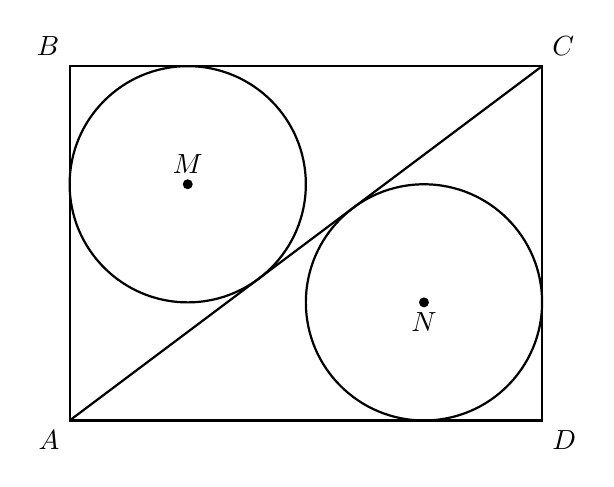
\begin{tikzpicture}[scale=1.5, thick]
        % Coordinates
        \coordinate (A) at (0,0);
        \coordinate (B) at (0,3);
        \coordinate (C) at (4,3);
        \coordinate (D) at (4,0);
        \coordinate (M) at (1,2);
        \coordinate (N) at (3,1);
    
        % Draw rectangle and diagonal
        \draw (A) -- (B) -- (C) -- (D) -- cycle;
        \draw (A) -- (C);
    
        % Draw inscribed circles
        \draw (M) circle (1);
        \draw (N) circle (1);
    
        % Draw centers and labels
        \fill (M) circle (1.2pt) node[above] {$M$};
        \fill (N) circle (1.2pt) node[below] {$N$};
    
        % Draw corner labels
        \node[below left] at (A) {$A$};
        \node[above left] at (B) {$B$};
        \node[above right] at (C) {$C$};
        \node[below right] at (D) {$D$};
    \end{tikzpicture}
    \end{center}
    \begin{itemize}
        \item[(A)] 2
        \item[(B)] 3
        \item[(C)] 4
        \item[(D)] 5
        \item[(E)] 6
    \end{itemize}

    % 16. E
    \item Sebuah belah ketupat memiliki tinggi 15 dan diagonal dengan rasio panjang 3:4. Berapakah panjang diagonal terpanjang dari belah ketupat tersebut?
    \begin{itemize}
        \item[(A)] 10
        \item[(B)] $\frac{25}{2}$
        \item[(C)] 15
        \item[(D)] 20
        \item[(E)] 25
    \end{itemize}

    % 17. E
    \item Kelas Prasekolah WOOT Pak Mebane sedang mengambil foto kelas. Ada lima anak laki-laki di kelas, dan tinggi mereka adalah 48, 49, 50, 51, dan 52 inci. Dalam foto kelas, mereka akan duduk di lima kursi yang disusun dalam satu baris. Berapa banyak cara siswa Pak Mebane dapat menduduki kursi tersebut sehingga tidak ada anak laki-laki yang duduk di sebelah anak laki-laki lain yang tingginya tepat satu inci lebih tinggi darinya?
    \begin{itemize}
        \item[(A)] 6
        \item[(B)] 8
        \item[(C)] 10
        \item[(D)] 12
        \item[(E)] 14
    \end{itemize}

    % 18. C
    \item Definisikan barisan $\{a_{k}\}$ sedemikian sehingga $a_{k}=1!+2!+3!+\dots+k!$ untuk setiap bilangan bulat positif $k$. Untuk berapa banyak bilangan bulat positif $1\le n\le 2013$ sehingga kuantitas $a_{1}+a_{2}+a_{3}+\dots+a_{n}$ berakhiran dengan digit 3?
    \begin{itemize}
        \item[(A)] 100
        \item[(B)] 201
        \item[(C)] 202
        \item[(D)] 203
        \item[(E)] 403
    \end{itemize}

    % 19. C
    \item Untuk setiap bilangan bulat positif $n$, misalkan $a_{n}=\frac{n^{2}}{2n+1}$. Selanjutnya, misalkan $P$ dan $Q$ adalah bilangan riil sedemikian sehingga $P=a_{1}a_{2}\dots a_{2013}$ and $Q=(a_{1}+1)(a_{2}+1)\dots(a_{2013}+1)$. Berapakah jumlah digit-digit dari $\lfloor\frac{Q}{P}\rfloor$?
    \begin{itemize}
        \item[(A)] 27
        \item[(B)] 29
        \item[(C)] 31
        \item[(D)] 33
        \item[(E)] 35
    \end{itemize}

    % 20. A
    \item Salah satu adegan yang dihapus dari film Inception melibatkan sebuah persegi yang menggantung di udara pada sudut tertentu. Ellen mampu memperpanjang sisi-sisi persegi tersebut hingga menyentuh tanah pada titik-titik $P, A, G,$ and $E$ sesuai urutan tersebut. Pengukuran sederhana menunjukkan bahwa $PA=2$ and $GE=3$. Berapakah luas persegi tersebut?
    \begin{itemize}
        \item[(A)] $\frac{36}{13}$
        \item[(B)] 3
        \item[(C)] $\frac{48}{13}$
        \item[(D)] $\frac{23}{4}$
        \item[(E)] 4
    \end{itemize}

    % 21. D
    \item Pada $\triangle ABC$, $AB=13$, $AC=14$, and $BC=15$. Misalkan $M$ melambangkan titik tengah $\overline{AC}$. Titik $P$ diletakkan pada segmen garis $\overline{BM}$ sedemikian sehingga $\overline{AP}\perp\overline{PC}$. Misalkan $p, q,$ and $r$ adalah bilangan bulat positif dengan $p$ and $r$ relatif prima dan $q$ bebas kuadrat sedemikian sehingga luas $\triangle APC$ dapat ditulis dalam bentuk $\frac{p\sqrt{q}}{r}$. Berapakah $p+q+r$?
    \begin{itemize}
        \item[(A)] 221
        \item[(B)] 257
        \item[(C)] 302
        \item[(D)] 368
        \item[(E)] 391
    \end{itemize}

    % 22. A
    \item Lima timbangan berat, dilabeli A, B, C, D, dan E, diletakkan bersisian di atas meja. Richard ingin mendistribusikan delapan beban identik seberat 5 ons di antara kelima timbangan ini. Namun, jika berat gabungan pada salah satu timbangan melebihi 15 ons, timbangan tersebut akan rusak. Ada berapa banyak cara Richard dapat mendistribusikan beban tersebut sehingga tidak ada satu pun dari kelima timbangan yang rusak?
    \begin{itemize}
        \item[(A)] 155
        \item[(B)] 160
        \item[(C)] 165
        \item[(D)] 175
        \item[(E)] 190
    \end{itemize}

    % 23. E
    \item Sebuah bilangan bulat dikatakan "terpisah-dua" jika dapat dinyatakan sebagai hasil kali dua bilangan bulat positif yang berselisih dua. Demikian pula, sebuah bilangan bulat dikatakan "terpisah-sembilan" jika dapat dinyatakan sebagai hasil kali dua bilangan bulat positif yang berselisih 9. Berapakah jumlah dari semua bilangan bulat positif yang merupakan terpisah-dua sekaligus terpisah-sembilan?
    \begin{itemize}
        \item[(A)] 460
        \item[(B)] 424
        \item[(C)] 396
        \item[(D)] 375
        \item[(E)] 360
    \end{itemize}

    % 24. A
    \item Berapa banyak himpunan bagian $A$ dan $B$ yang saling lepas dari $\{1, 2, 3, 4, 5, 6, 7, 8\}$ sedemikian sehingga $|A|+|B|\in A$ dan $|A|-|B|\in B$?
    \begin{itemize}
        \item[(A)] 294
        \item[(B)] 316
        \item[(C)] 342
        \item[(D)] 363
        \item[(E)] 375
    \end{itemize}

    % 25. B
    \item Misalkan $P(x)=(x^{2}-x+1)(x^{4}-x^{2}+1)(x^{8}-x^{4}+1)\dots(x^{1024}-x^{512}+1)$. Ketika $P(x)$ dijabarkan, ada berapa banyak suku yang dikandungnya?
    \begin{itemize}
        \item[(A)] 1025
        \item[(B)] 1365
        \item[(C)] 1679
        \item[(D)] 1885
        \item[(E)] 2043
    \end{itemize}
\end{enumerate}

\end{document}

\end{document}
% \documentclass[11pt]{article}
% \usepackage[utf8]{inputenc}
% \usepackage{amsmath}
% \usepackage{amsfonts}
% \usepackage{amssymb}
% \usepackage{geometry}
% \geometry{a4paper, margin=1in}

% \begin{document}
% % https://cdn.artofproblemsolving.com/attachments/6/7/bfa80c21829e4268c5e82d86dfec05d701d40f
% \section*{Mock AMC 10 Questions}

% \begin{enumerate}
%     \item What is the value of $\frac{1+2+3}{2+3+4}+\frac{3+4+5}{4+5+6}$?
%     \begin{itemize}
%         \item[(A)] $\frac{5}{4}$
%         \item[(B)] $\frac{22}{15}$
%         \item[(C)] $\frac{25}{12}$
%         \item[(D)] $\frac{147}{60}$
%         \item[(E)] $\frac{5}{2}$
%     \end{itemize}

%     \item Through an online internet service named Likes, the amount of money in Sam's back account increases by \$0.03 for every person who accesses his page through a link. Suppose that at midnight on Monday Sam's account was worth \$10.56, and by midnight on Tuesday Sam's account was worth \$11.25. How many people clicked on Sam's link on Monday?
%     \begin{itemize}
%         \item[(A)] 15
%         \item[(B)] 18
%         \item[(C)] 20
%         \item[(D)] 22
%         \item[(E)] 23
%     \end{itemize}

%     \item Suppose that $x$ is a real number such that $7x+19=2013$. What is $7x-19$?
%     \begin{itemize}
%         \item[(A)] 1971
%         \item[(B)] 1973
%         \item[(C)] 1975
%         \item[(D)] 1977
%         \item[(E)] 1994
%     \end{itemize}

%     \item The ratio of the area of a circle to the circumference of the same circle is 6. What is the radius of the circle?
%     \begin{itemize}
%         \item[(A)] $6\pi$
%         \item[(B)] 12
%         \item[(C)] 6
%         \item[(D)] 3
%         \item[(E)] $\frac{6}{\pi}$
%     \end{itemize}

%     \item How many positive integers from 1 to 1000 have an odd number of digits?
%     \begin{itemize}
%         \item[(A)] 500
%         \item[(B)] 700
%         \item[(C)] 900
%         \item[(D)] 909
%         \item[(E)] 1000
%     \end{itemize}

%     \item Define an ordered triplet of positive integers $(a, b, c)$ to be triangular if it is possible to construct a triangle with side lengths $a, b,$ and $c$. What is the maximum value of $x+y$ if the ordered triplet $(5, x, y)$ is triangular, given that $x \le 20$ and $y \le 13$?
%     \begin{itemize}
%         \item[(A)] 28
%         \item[(B)] 29
%         \item[(C)] 30
%         \item[(D)] 31
%         \item[(E)] 32
%     \end{itemize}

%     \item The probability that it will rain on any given day is 30\%. What is the probability that it will rain on exactly one of two consecutive days?
%     \begin{itemize}
%         \item[(A)] 15\%
%         \item[(B)] 21\%
%         \item[(C)] 30\%
%         \item[(D)] 42\%
%         \item[(E)] 50\%
%     \end{itemize}

%     \item A certain number of people attended a mathematics convention. Of the total attendees, $\frac{3}{5}$ of them participated in a math competition; $\frac{15}{22}$ of the remaining instead decided to listen to a seminar on Topology. What is the smallest possible number of attendees that neither participated in the competition nor listened to the lecture?
%     \begin{itemize}
%         \item[(A)] 5
%         \item[(B)] 7
%         \item[(C)] 14
%         \item[(D)] 15
%         \item[(E)] 22
%     \end{itemize}

%     \item Let $p$ and $q$ be real numbers with $|p|<1$ and $|q|<1$ such that
%     \[p+pq+pq^{2}+pq^{3}+\dots=2\]
%     \[q+qp+qp^{2}+qp^{3}+\dots=3\]
%     What is $100pq$?
%     \begin{itemize}
%         \item[(A)] 24
%         \item[(B)] 32
%         \item[(C)] 36
%         \item[(D)] 40
%         \item[(E)] 48
%     \end{itemize}

%     \item A regular 2013-gon is placed in the plane in general position. A family of lines is drawn on this plane such that no two lines are parallel, and for every vertex $A$ of the 2013-gon, there exists a line that passes through $A$. What is the smallest number of possible lines in the family?
%     \begin{itemize}
%         \item[(A)] 504
%         \item[(B)] 1006
%         \item[(C)] 1007
%         \item[(D)] 2012
%         \item[(E)] 2013
%     \end{itemize}

%     \item In a small private science-oriented school, there are eight classes to choose from: Earth Systems, Biology, Chemistry, Physics, Art, Music, History, and Spanish. David is trying to fill his four-period schedule with classes. He can take at most three science courses, and he has to take exactly one of art or music. If the order of the courses does not matter, how many possible schedules can David make?
%     \begin{itemize}
%         \item[(A)] 40
%         \item[(B)] 44
%         \item[(C)] 48
%         \item[(D)] 52
%         \item[(E)] 56
%     \end{itemize}

%     \item Suppose $a$ and $b$ are real numbers that satisfy the system of equations
%     \begin{align*}
%     a+b &= 9 \\
%     a(a-2)+b(b-2) &= 21
%     \end{align*}
%     What is $ab$?
%     \begin{itemize}
%         \item[(A)] 15
%         \item[(B)] 20
%         \item[(C)] 21
%         \item[(D)] 25
%         \item[(E)] 27
%     \end{itemize}

%     \item Rectangle $ABCD$ has $AB=5$ and $BC=12$. $CD$ is extended to a point $E$ such that $\triangle ACE$ is isosceles with base $AC$. What is the area of triangle $ADE$?
%     \begin{itemize}
%         \item[(A)] 15
%         \item[(B)] $\frac{131}{5}$
%         \item[(C)] 30
%         \item[(D)] $\frac{357}{5}$
%         \item[(E)] 125
%     \end{itemize}

%     \item Rachel went to the local convenience store to buy some packs of seeds. In the convenience store, large packs cost \$1.35 apiece and small packs cost \$0.85 apiece. If Rachel paid \$20.15 for her order, which type of pack did she buy more of, and by how many?
%     \begin{itemize}
%         \item[(A)] 1 more small pack
%         \item[(B)] 2 more small packs
%         \item[(C)] 3 more small packs
%         \item[(D)] 1 more large pack
%         \item[(E)] 2 more large packs
%     \end{itemize}

%     \item Let $ABCD$ be a rectangle such that $AB=3$ and $BC=4$. Suppose that $M$ and $N$ are the centers of the circles inscribed inside triangles $\triangle ABC$ and $\triangle ADC$ respectively. What is $MN^{2}$?
    \begin{center}
        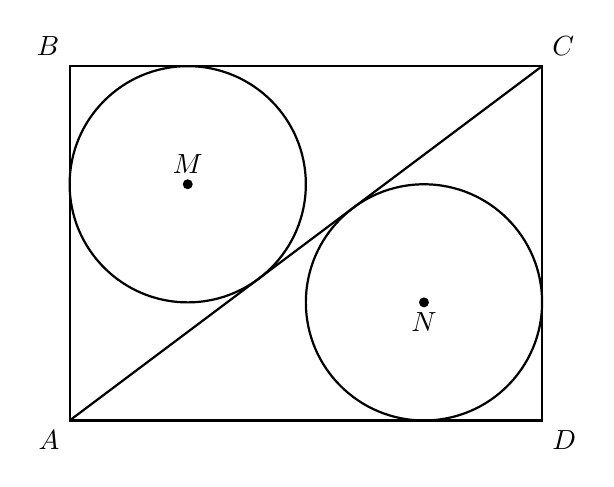
\begin{tikzpicture}[scale=1.5, thick]
        % Coordinates
        \coordinate (A) at (0,0);
        \coordinate (B) at (0,3);
        \coordinate (C) at (4,3);
        \coordinate (D) at (4,0);
        \coordinate (M) at (1,2);
        \coordinate (N) at (3,1);
    
        % Draw rectangle and diagonal
        \draw (A) -- (B) -- (C) -- (D) -- cycle;
        \draw (A) -- (C);
    
        % Draw inscribed circles
        \draw (M) circle (1);
        \draw (N) circle (1);
    
        % Draw centers and labels
        \fill (M) circle (1.2pt) node[above] {$M$};
        \fill (N) circle (1.2pt) node[below] {$N$};
    
        % Draw corner labels
        \node[below left] at (A) {$A$};
        \node[above left] at (B) {$B$};
        \node[above right] at (C) {$C$};
        \node[below right] at (D) {$D$};
    \end{tikzpicture}
    \end{center}
%     \begin{itemize}
%         \item[(A)] 2
%         \item[(B)] 3
%         \item[(C)] 4
%         \item[(D)] 5
%         \item[(E)] 6
%     \end{itemize}

%     \item A rhombus has height 15 and diagonals with lengths in a ratio of 3:4. What is the length of the longer diagonal of the rhombus?
%     \begin{itemize}
%         \item[(A)] 10
%         \item[(B)] $\frac{25}{2}$
%         \item[(C)] 15
%         \item[(D)] 20
%         \item[(E)] 25
%     \end{itemize}

%     \item Mr. Mebane's Preschool WOOT class is taking a class photograph. There are five boys in the class, and they are 48, 49, 50, 51, and 52 inches tall. In the class photograph, they are to sit themselves in five chairs positioned in a row. In how many ways can Mr. Mebane's students seat themselves such that no boy sits next to another boy who is exactly one inch taller than himself?
%     \begin{itemize}
%         \item[(A)] 6
%         \item[(B)] 8
%         \item[(C)] 10
%         \item[(D)] 12
%         \item[(E)] 14
%     \end{itemize}

%     \item Define the sequence $\{a_{k}\}$ such that $a_{k}=1!+2!+3!+\dots+k!$ for each positive integer $k$. For how many positive integers $1\le n\le 2013$ does the quantity $a_{1}+a_{2}+a_{3}+\dots+a_{n}$ end in the digit 3?
%     \begin{itemize}
%         \item[(A)] 100
%         \item[(B)] 201
%         \item[(C)] 202
%         \item[(D)] 203
%         \item[(E)] 403
%     \end{itemize}

%     \item For each positive integer $n$, let $a_{n}=\frac{n^{2}}{2n+1}$. Furthermore, let $P$ and $Q$ be real numbers such that $P=a_{1}a_{2}\dots a_{2013}$ and $Q=(a_{1}+1)(a_{2}+1)\dots(a_{2013}+1)$. What is the sum of the digits of $\lfloor\frac{Q}{P}\rfloor$?
%     \begin{itemize}
%         \item[(A)] 27
%         \item[(B)] 29
%         \item[(C)] 31
%         \item[(D)] 33
%         \item[(E)] 35
%     \end{itemize}

%     \item One deleted scene from the movie Inception involved a square hanging in mid-air at a certain angle. Ellen was able to extend the sides of the square until they met the ground at points $P, A, G,$ and $E$ in that order. Simple measurements showed that $PA=2$ and $GE=3$. What was the area of the square?
%     \begin{itemize}
%         \item[(A)] $\frac{36}{13}$
%         \item[(B)] 3
%         \item[(C)] $\frac{48}{13}$
%         \item[(D)] $\frac{23}{4}$
%         \item[(E)] 4
%     \end{itemize}

%     \item In $\triangle ABC$, $AB=13$, $AC=14$, and $BC=15$. Let $M$ denote the midpoint of $\overline{AC}$. Point $P$ is placed on line segment $\overline{BM}$ such that $\overline{AP}\perp\overline{PC}$. Suppose that $p, q,$ and $r$ are positive integers with $p$ and $r$ relatively prime and $q$ squarefree such that the area of $\triangle APC$ can be written in the form $\frac{p\sqrt{q}}{r}$. What is $p+q+r$?
%     \begin{itemize}
%         \item[(A)] 221
%         \item[(B)] 257
%         \item[(C)] 302
%         \item[(D)] 368
%         \item[(E)] 391
%     \end{itemize}

%     \item Five weight scales, labeled A, B, C, D, and E, are placed side-by-side on a table. Richard wants to distribute eight identical 5 ounce weights among these five scales. However, if the combined weight on any one of the scales exceeds 15 ounces, the scale will break. In how many ways can Richard distribute the weights such that none of the five scales collapse?
%     \begin{itemize}
%         \item[(A)] 155
%         \item[(B)] 160
%         \item[(C)] 165
%         \item[(D)] 175
%         \item[(E)] 190
%     \end{itemize}

%     \item An integer is said to be two-separable if it can be represented as the product of two positive integers that differ by two. Similarly, an integer is said to be nine-separable if it can be represented as the product of two positive integers that differ by 9. What is the sum of all positive integers that are both two-separable and nine-separable?
%     \begin{itemize}
%         \item[(A)] 460
%         \item[(B)] 424
%         \item[(C)] 396
%         \item[(D)] 375
%         \item[(E)] 360
%     \end{itemize}

%     \item How many disjoint subsets $A$ and $B$ of $\{1, 2, 3, 4, 5, 6, 7, 8\}$ are there such that $|A|+|B|\in A$ and $|A|-|B|\in B$?
%     \begin{itemize}
%         \item[(A)] 294
%         \item[(B)] 316
%         \item[(C)] 342
%         \item[(D)] 363
%         \item[(E)] 375
%     \end{itemize}

%     \item Let $P(x)=(x^{2}-x+1)(x^{4}-x^{2}+1)(x^{8}-x^{4}+1)\dots(x^{1024}-x^{512}+1)$. When $P(x)$ is expanded, how many terms does it contain?
%     \begin{itemize}
%         \item[(A)] 1025
%         \item[(B)] 1365
%         \item[(C)] 1679
%         \item[(D)] 1885
%         \item[(E)] 2043
%     \end{itemize}
% \end{enumerate}

% \end{document}